\documentclass[a4paper,11pt]{book}

\author{Sebastian Pancratz}
\title{Practical improvements to the deformation method for point counting}

%%%%%%%%%%%%%%%%%%%%%%%%%%%%%%%%%%%%%%%%%%%%%%%%%%%%%%%%%%%%%%%%%%%%%%%%%%%%%%%
% Geometry and page layout

\usepackage[hmargin=2.2cm,vmargin=3cm,a4paper,centering,twoside]{geometry}

\setlength{\headheight}{14pt}

%%%%%%%%%%%%%%%%%%%%%%%%%%%%%%%%%%%%%%%%%%%%%%%%%%%%%%%%%%%%%%%%%%%%%%%%%%%%%%%
% Other packages

\usepackage{ifpdf}
\usepackage{paralist}
\usepackage{fancyhdr}
\usepackage{sectsty}
\usepackage{natbib}
\usepackage{url}
\usepackage[T1]{fontenc}
\usepackage{ae,aecompl}
\usepackage{booktabs}
\usepackage{multirow}
\usepackage{verbatim}

\usepackage{float}
\usepackage{tikz}
\usetikzlibrary{shapes,arrows}

%%%%%%%%%%%%%%%%%%%%%%%%%%%%%%%%%%%%%%%%%%%%%%%%%%%%%%%%%%%%%%%%%%%%%%%%%%%%%%%
% hyperref

\usepackage{hyperref}
\hypersetup{
    colorlinks=true,    % false: boxed links; true: colored links
    citecolor=green,    % color of links to bibliography
    filecolor=magenta,  % color of file links
    linkcolor=red,      % color of internal links
    urlcolor=blue       % color of external links
}

\makeatletter
\newcommand\org@hypertarget{}
\let\org@hypertarget\hypertarget
\renewcommand\hypertarget[2]{%
    \Hy@raisedlink{\org@hypertarget{#1}{}}#2%
} 
\makeatother

\ifpdf
    \hypersetup{
        pdftitle={Deformation method},
        pdfauthor={Sebastian Pancratz},
        pdfsubject={Computational Number Theory},
        bookmarks=true,
        bookmarksnumbered=true,
        unicode=true,
        pdfstartview={FitH},
        pdfpagemode={UseOutlines}
    }
\fi

%%%%%%%%%%%%%%%%%%%%%%%%%%%%%%%%%%%%%%%%%%%%%%%%%%%%%%%%%%%%%%%%%%%%%%%%%%%%%%%
% natbib

\bibpunct{[}{]}{,}{n}{}{}
%\bibpunct{[}{]}{;}{a}{,}{,}

%%%%%%%%%%%%%%%%%%%%%%%%%%%%%%%%%%%%%%%%%%%%%%%%%%%%%%%%%%%%%%%%%%%%%%%%%%%%%%%
% sectsty

\allsectionsfont{\nohang\centering}

%%%%%%%%%%%%%%%%%%%%%%%%%%%%%%%%%%%%%%%%%%%%%%%%%%%%%%%%%%%%%%%%%%%%%%%%%%%%%%%
% fancyhdr

\newcommand\nouppercase[1]{{%
    \let\uppercase\relax
    \let\MakeUppercase\relax
    \expandafter\let\csname MakeUppercase \endcsname\relax#1}%
}

\pagestyle{fancyplain}

\renewcommand{\chaptermark}[1]{\markboth{#1}{}}
\renewcommand{\sectionmark}[1]{\markright{\thesection\ #1}}
\fancyhf{}
\fancyhead[LE,RO]{\bfseries\thepage}
\fancyhead[LO]{\itshape\nouppercase{\rightmark}}
\fancyhead[RE]{\itshape\nouppercase{\leftmark}}
\renewcommand{\headrulewidth}{0pt}
\renewcommand{\footrulewidth}{0pt}

\fancypagestyle{plain}{%
  \fancyhead{}
  \renewcommand{\headrulewidth}{0pt}
}

\makeatletter
\def\cleardoublepage{\clearpage\if@twoside \ifodd\c@page\else
    \hbox{}
    \thispagestyle{plain}
    \newpage
    \if@twocolumn\hbox{}\newpage\fi\fi\fi}
\makeatother \clearpage{\pagestyle{plain}\cleardoublepage}

%%%%%%%%%%%%%%%%%%%%%%%%%%%%%%%%%%%%%%%%%%%%%%%%%%%%%%%%%%%%%%%%%%%%%%%%%%%%%%%
% url

\makeatletter
\def\url@leostyle{%
  \@ifundefined{selectfont}{\def\UrlFont{\sf}}{\def\UrlFont{\small\ttfamily}}}
\makeatother
\urlstyle{leostyle}

%%%%%%%%%%%%%%%%%%%%%%%%%%%%%%%%%%%%%%%%%%%%%%%%%%%%%%%%%%%%%%%%%%%%%%%%%%%%%%%
% Enumeration

\setlength{\pltopsep}{0.24em}
\setlength{\plpartopsep}{0em}
\setlength{\plitemsep}{0.24em}

% This should do what we want
%   \setdefaultenum{(i)}{(a)}{1.}{A}
% but it does not work for references, dropping the parentheses.  The following
% hack does work.

\renewcommand{\theenumi}{(\roman{enumi})}
\renewcommand{\theenumii}{(\alph{enumii})}
\renewcommand{\theenumiii}{\arabic{enumiii}.}
\renewcommand{\theenumiv}{\Alph{enumiv}}

\renewcommand{\labelenumi}{\theenumi}
\renewcommand{\labelenumii}{\theenumii}
\renewcommand{\labelenumiii}{\theenumiii}
\renewcommand{\labelenumiv}{\theenumiv}

%%%%%%%%%%%%%%%%%%%%%%%%%%%%%%%%%%%%%%%%%%%%%%%%%%%%%%%%%%%%%%%%%%%%%%%%%%%%%%%
% Bibliography name

\renewcommand{\bibname}{References}

%%%%%%%%%%%%%%%%%%%%%%%%%%%%%%%%%%%%%%%%%%%%%%%%%%%%%%%%%%%%%%%%%%%%%%%%%%%%%%%
% Mathematical definitions

%%%%%%%%%%%%%%%%%%%%%%%%%%%%%%%%%%%%%%%%%%%%%%%%%%%%%%%%%%%%%%%%%%%%%%%%%%%%%%%
% A selection of mathematical commands for inclusion in a LaTeX document.
% 
% Author.  Sebastian Pancratz
% Date.    Nov 2009

%%%%%%%%%%%%%%%%%%%%%%%%%%%%%%%%%%%%%%%%%%%%%%%%%%%%%%%%%%%%%%%%%%%%%%%%%%%%%%%
% Packages

\usepackage{amsmath,amsthm,amscd,amsfonts,amssymb}
\usepackage{cases}
\usepackage[all]{xy}

%%%%%%%%%%%%%%%%%%%%%%%%%%%%%%%%%%%%%%%%%%%%%%%%%%%%%%%%%%%%%%%%%%%%%%%%%%%%%%%
% General Mathematics

\newcommand{\myland}{\mspace{6mu} \land \mspace{6mu}}%  logical and
\newcommand{\mylor}{\mspace{6mu} \lor \mspace{6mu}}%    logical or

\renewcommand{\to}{\rightarrow}%           Right arrow
\newcommand{\into}{\hookrightarrow}%     Injection arrow
\newcommand{\onto}{\twoheadrightarrow}%  Surjection arrow

\providecommand{\card}[1]{\left\lvert#1\right\rvert}%    Cardinality
\providecommand{\cardts}[1]{\lvert#1\rvert}%             Cardinality
\providecommand{\cardbig}[1]{\bigl\lvert#1\bigr\rvert}%  Cardinality

\providecommand{\abs}[1]{\lvert#1\rvert}%                  Absolute value
\providecommand{\absbig}[1]{\bigl\lvert#1\bigr\rvert}%     Absolute value
\providecommand{\absBig}[1]{\Bigl\lvert#1\Bigr\rvert}%     Absolute value
\providecommand{\absbigg}[1]{\biggl\lvert#1\biggr\rvert}%  Absolute value

\providecommand{\norm}[1]{\lVert#1\rVert}%               Norm
\providecommand{\normbig}[1]{\bigl\lVert#1\bigr\rVert}%  Norm
\providecommand{\normBig}[1]{\Bigl\lVert#1\Bigr\rVert}%  Norm

\providecommand{\floor}[1]{\left\lfloor#1\right\rfloor}%    Floor
\providecommand{\floorts}[1]{\lfloor#1\rfloor}%             Floor
\providecommand{\floorbig}[1]{\bigl\lfloor#1\bigr\rfloor}%  Floor
\providecommand{\floorBig}[1]{\Bigl\lfloor#1\Bigr\rfloor}%  Floor

\providecommand{\ceil}[1]{\left\lceil#1\right\rceil}%  Ceiling

\providecommand{\id}{\iota}%              Identity element or function
\DeclareMathOperator{\ind}{1}%            Indicator function
\DeclareMathOperator{\indf}{\mathbf{1}}%  Indicator function

\DeclareMathOperator{\fCoKer}{coker}%  Cokernel
\DeclareMathOperator{\fKer}{ker}%      Kernel
\DeclareMathOperator{\fIm}{Im}%        Image

\DeclareMathOperator{\Comb}{C}%  Combinations
\DeclareMathOperator{\Perm}{P}%  Permutations

%%%%%%%%%%%%%%%%%%%%%%%%%%%%%%%%%%%%%%%%%%%%%%%%%%%%%%%%%%%%%%%%%%%%%%%%%%%%%%%
% Commonly used Sets

\newcommand{\N}{\mathbf{N}}%  Natural numbers
\newcommand{\Z}{\mathbf{Z}}%  Integers
\newcommand{\Q}{\mathbf{Q}}%  Rationals
\newcommand{\A}{\mathbf{A}}%  Algebraic numbers
\newcommand{\R}{\mathbf{R}}%  Real numbers
\providecommand{\C}{\mathbf{C}}%  Complex numbers
\newcommand{\F}{\mathbf{F}}%  Finite field

\let\P=\undefined
\newcommand{\P}{\mathbf{P}}%  Projective space, N.B.  Clashes with Probability

%%%%%%%%%%%%%%%%%%%%%%%%%%%%%%%%%%%%%%%%%%%%%%%%%%%%%%%%%%%%%%%%%%%%%%%%%%%%%%%
% Probability

%\let\P=\undefined

\DeclareMathOperator{\E}{\mathbb{E}}%  Expectation
%\DeclareMathOperator{\P}{\mathbb{P}}%  Probability
\DeclareMathOperator{\Var}{Var}%       Variance
\DeclareMathOperator{\Cov}{Cov}%       Covariance
\DeclareMathOperator{\Corr}{Corr}%     Correlation

%%%%%%%%%%%%%%%%%%%%%%%%%%%%%%%%%%%%%%%%%%%%%%%%%%%%%%%%%%%%%%%%%%%%%%%%%%%%%%%
% Algebraic Topology

\DeclareMathOperator{\rel}{rel}
\providecommand{\GeoReal}[1]{\abs{#1}}
\DeclareMathOperator{\Star}{star}
\DeclareMathOperator{\mesh}{mesh}

%%%%%%%%%%%%%%%%%%%%%%%%%%%%%%%%%%%%%%%%%%%%%%%%%%%%%%%%%%%%%%%%%%%%%%%%%%%%%%%
% Complex Analysis

\providecommand{\wn}{\omega}%  Winding number

%%%%%%%%%%%%%%%%%%%%%%%%%%%%%%%%%%%%%%%%%%%%%%%%%%%%%%%%%%%%%%%%%%%%%%%%%%%%%%%
% Galois Theory

\DeclareMathOperator{\Disc}{Disc}%      Discriminant
\DeclareMathOperator{\ch}{char}%        Characteristic
\DeclareMathOperator{\geomCirc}{circ}%  Circle for ruler & compass constructions
\DeclareMathOperator{\Gal}{Gal}%        Galois group

%%%%%%%%%%%%%%%%%%%%%%%%%%%%%%%%%%%%%%%%%%%%%%%%%%%%%%%%%%%%%%%%%%%%%%%%%%%%%%%
% Graph Theory

\providecommand{\E}{\mathbb{E}}%  Edge space
\providecommand{\V}{\mathbb{V}}%  Vertex space
\DeclareMathOperator{\ex}{ex}%    Maximal size of a graph such that it does not have a given subgraph

%%%%%%%%%%%%%%%%%%%%%%%%%%%%%%%%%%%%%%%%%%%%%%%%%%%%%%%%%%%%%%%%%%%%%%%%%%%%%%%
% Groups, Rings and Modules

\providecommand{\subgrp}{\leq}%           Subgroup
\providecommand{\normal}{\triangleleft}%  Normal subgroup
\providecommand{\subring}{\leq}%          Subring
\providecommand{\ideal}{\triangleleft}%   Ideal
\providecommand{\submodule}{\leq}%        Submodule

\DeclareMathOperator{\Sym}{Sym}%      Symmetric group
\DeclareMathOperator{\Aut}{Aut}%      Automorphism group
\DeclareMathOperator{\ccl_G}{ccl_G}%  Conjugacy class
\DeclareMathOperator{\Ann}{Ann}%      Annihilator
\DeclareMathOperator{\sgn}{sgn}%      Sign, signature
\DeclareMathOperator{\stab}{Stab}%    Stabiliser

%%%%%%%%%%%%%%%%%%%%%%%%%%%%%%%%%%%%%%%%%%%%%%%%%%%%%%%%%%%%%%%%%%%%%%%%%%%%%%%
% Linear Algebra, Linear Analysis

\providecommand{\vect}[1]{\mathbf{#1}}%                       Vector
\providecommand{\vspan}[1]{\langle #1 \rangle}%               Span
\providecommand{\iprod}[2]{\langle #1,#2 \rangle}%            Inner product
\providecommand{\ip}[2]{\left\langle #1 , #2 \right\rangle}%  Inner product

\DeclareMathOperator{\rank}{rank}%       Rank of a matrix
\DeclareMathOperator{\vsspan}{span}%     Span
\DeclareMathOperator{\diag}{diag}%       Diagonal matrix
\DeclareMathOperator{\rowrank}{rowrk}%   Row rank
\DeclareMathOperator{\colspace}{colsp}%  Column space
\DeclareMathOperator{\rowspace}{rowsp}%  Column space
\DeclareMathOperator{\adj}{adj}%         Adjoint matrix
\DeclareMathOperator{\trace}{tr}%        Trace
\DeclareMathOperator{\End}{End}%         Space of endomorphisms
\DeclareMathOperator{\SL}{SL}%           Special linear group of matrices

%%%%%%%%%%%%%%%%%%%%%%%%%%%%%%%%%%%%%%%%%%%%%%%%%%%%%%%%%%%%%%%%%%%%%%%%%%%%%%%
% Metric and Topological Spaces

\DeclareMathOperator{\diam}{diam}%  Diameter
\DeclareMathOperator{\Int}{int}%    Interior of a set
\DeclareMathOperator{\Cl}{cl}%      Closure of a set

%%%%%%%%%%%%%%%%%%%%%%%%%%%%%%%%%%%%%%%%%%%%%%%%%%%%%%%%%%%%%%%%%%%%%%%%%%%%%%%
% Number Theory

\providecommand{\jacobi}[2]{\left( \frac{#1}{#2} \right)}%    Jacobi symbol (display)
\providecommand{\jacobii}[2]{\left( #1 \vert #2 \right)}%     Jacobi symbol (inline)
\providecommand{\legendre}[2]{\left( \frac{#1}{#2} \right)}%  Legendre symbol (display)
\providecommand{\legendrei}[2]{\left( #1 \vert #2 \right)}%   Legendre symbol (inline)

\DeclareMathOperator{\hcf}{hcf}%  Highest common factor
\DeclareMathOperator{\lcm}{lcm}%  Lowest common multiple

%%%%%%%%%%%%%%%%%%%%%%%%%%%%%%%%%%%%%%%%%%%%%%%%%%%%%%%%%%%%%%%%%%%%%%%%%%%%%%%
% Local Fields

\newcommand{\ilim}{\varprojlim}%  inverse limit

\DeclareMathOperator{\ord}{ord}%          Valuation
\DeclareMathOperator{\Frac}{Frac}%        Field of fractions
\DeclareMathOperator{\Frob}{\mathcal{F}}% Frobenius map
\DeclareMathOperator{\Hom}{Hom}%          Space of homomorphisms
\DeclareMathOperator{\Tr}{Tr}%            Trace

%%%%%%%%%%%%%%%%%%%%%%%%%%%%%%%%%%%%%%%%%%%%%%%%%%%%%%%%%%%%%%%%%%%%%%%%%%%%%%%
% Algebraic Geometry

\DeclareMathOperator{\Spec}{Spec}%  Spectrum

%%%%%%%%%%%%%%%%%%%%%%%%%%%%%%%%%%%%%%%%%%%%%%%%%%%%%%%%%%%%%%%%%%%%%%%%%%%%%%%
% Calligraphic letters

\providecommand{\cB}{\mathcal{B}}%   Basis, factor base
\providecommand{\fC}{\mathfrak{C}}%  Codes
\providecommand{\cS}{\mathcal{S}}%   Signatures
\providecommand{\cK}{\mathfrak{K}}%  Keys
\providecommand{\cM}{\mathfrak{M}}%  Messages
\providecommand{\cE}{\mathcal{E}}%   (See error locator polynomial)
\providecommand{\cF}{\mathcal{F}}%   Family
\providecommand{\cO}{\mathcal{O}}%   Big-oh notation
\providecommand{\cP}{\mathcal{P}}%   Power set
\providecommand{\cR}{\mathcal{R}}%   Row index set
\providecommand{\cC}{\mathcal{C}}%   Column index set


%%%%%%%%%%%%%%%%%%%%%%%%%%%%%%%%%%%%%%%%%%%%%%%%%%%%%%%%%%%%%%%%%%%%%%%%%%%%%%%
% Equations

\allowdisplaybreaks[4]
\numberwithin{equation}{chapter}

%%%%%%%%%%%%%%%%%%%%%%%%%%%%%%%%%%%%%%%%%%%%%%%%%%%%%%%%%%%%%%%%%%%%%%%%%%%%%%%
% Theorems etc

\theoremstyle{definition}

\newtheorem{thm}{Theorem}[section]
\newtheorem{lem}[thm]{Lemma}
\newtheorem{prop}[thm]{Proposition}
\newtheorem{cor}[thm]{Corollary}
\newtheorem{defn}[thm]{Definition}
\newtheorem{exmp}[thm]{Example}
\newtheorem{rem}[thm]{Remark}
\newtheorem{assumption}[thm]{Assumption}
\newtheorem{notation}[thm]{Notation}
\newtheorem{prob}[thm]{Problem}
\newtheorem{obs}[thm]{Observation}

%%%%%%%%%%%%%%%%%%%%%%%%%%%%%%%%%%%%%%%%%%%%%%%%%%%%%%%%%%%%%%%%%%%%%%%%%%%%%%%
% DOCUMENT                                                                    %
%%%%%%%%%%%%%%%%%%%%%%%%%%%%%%%%%%%%%%%%%%%%%%%%%%%%%%%%%%%%%%%%%%%%%%%%%%%%%%%

\begin{document}

\frontmatter

\tableofcontents

\mainmatter

{%
\part{The deformation method}
\setlength{\baselineskip}{1.5\baselineskip}
%%%%%%%%%%%%%%%%%%%%%%%%%%%%%%%%%%%%%%%%%%%%%%%%%%%%%%%%%%%%%%%%%%%%%%%%%%%%%%%
% Introduction to point counting                                              %
%%%%%%%%%%%%%%%%%%%%%%%%%%%%%%%%%%%%%%%%%%%%%%%%%%%%%%%%%%%%%%%%%%%%%%%%%%%%%%%

\chapter{Introduction to point counting}

%%%%%%%%%%%%%%%%%%%%%%%%%%%%%%%%%%%%%%%%%%%%%%%%%%%%%%%%%%%%%%%%%%%%%%%%%%%%%%%
% Geometric preliminaries                                                     %
%%%%%%%%%%%%%%%%%%%%%%%%%%%%%%%%%%%%%%%%%%%%%%%%%%%%%%%%%%%%%%%%%%%%%%%%%%%%%%%

\chapter{Geometric preliminaries}

%%%%%%%%%%%%%%%%%%%%%%%%%%%%%%%%%%%%%%%%%%%%%%%%%%%%%%%%%%%%%%%%%%%%%%%%%%%%%%%
% Introduction to the deformation method                                      %
%%%%%%%%%%%%%%%%%%%%%%%%%%%%%%%%%%%%%%%%%%%%%%%%%%%%%%%%%%%%%%%%%%%%%%%%%%%%%%%

\chapter{Introduction to the deformation method}

%%%%%%%%%%%%%%%%%%%%%%%%%%%%%%%%%%%%%%%%%%%%%%%%%%%%%%%%%%%%%%%%%%%%%%%%%%%%%%%
% Frobenius on the diagonal fibre                                             %
%%%%%%%%%%%%%%%%%%%%%%%%%%%%%%%%%%%%%%%%%%%%%%%%%%%%%%%%%%%%%%%%%%%%%%%%%%%%%%%

\chapter{Frobenius on the diagonal fibre}

In this chapter we discuss the action of Frobenius on the diagonal fibre. 
We first describe the general method based on an explicit formula by Dwork 
following the expositions in the work of Lauder~\citep[Section~6]{Lau04} 
and Gerkmann~\citep[Section~4.4]{Gerkmann2007}.  Then, we present a new 
improvement in Theorem~\ref{thm:alpha}, showing that a certain 
expression is defined already over $\mathbf{Q}_p$ instead of a ramified 
extension as observed by Gerkmann.  Furthermore, Theorems~\ref{thm:alpha2} 
and \ref{thm:alphap} state the expression lies in $\mathbf{Z}_p$ and 
provide computationally suitable reformulations.  To conclude this chapter, 
we illustrate the practical relevance of these improvements with two example 
computations.

% Introduction %%%%%%%%%%%%%%%%%%%%%%%%%%%%%%%%%%%%%%%%%%%%%%%%%%%%%%%%%%%%%%%%

\section{Introduction}

In order to simplify our notation, we temporarily suppress the earlier 
setup of a family of hypersurfaces.
Thus, we consider a smooth diagonal projective hypersurface~$X$ of degree~$d$ 
in $P^n(\mathbf{F}_q)$ and letting $U = P^n(\mathbf{F}_q) - X$ be the affine 
complement we aim to compute, to a prescribed precision~$N$, the matrix~$F$ 
representing the action of $q^{-1} F_q$ on 
$H_{rig}^n(U) \cong H_{dR}^n(\mathfrak{U})$ with respect to a specific 
monomial basis.  We recall that $n \geq 2$ and $d \geq 2$ whenever $n$ is odd 
and $d \geq 3$ whenever $n$ is even.

A smooth projective diagonal hypersurface $X$ over $\mathbf{F}_q$ 
is necessarily given by 
\begin{equation*}
P(x_0, x_1, \dotsc, x_n) = a_0 x_0^d + a_1 x_1^d + \dotsb + a_n x_n^d = 0
\end{equation*}
where $a_0, a_1, \dotsc, a_n \in \mathbf{F}_q^{\times}$ and $p \nmid d$.

We choose the basis $\mathcal{B}_1 \cup \dotsb \cup \mathcal{B}_n$ 
for $H_{dR}^n(\mathfrak{U})$ where, for $k = 1, \dotsc, n$, 
\begin{align*}
B_k & = \{ x^i : \text{$\abs{i} = kd - (n+1)$ and $0 \leq i_j < d-1$, for all $j$} \}, \\
\mathcal{B}_k & = \{x^i \Omega / P^k : x^i \in B_k \}.
\end{align*}

Let $F$ denote the matrix for $q^{-1} F_q$ on $H_{dR}^n(\mathfrak{U})$, 
where $F_q$ is the $q$-power Frobenius.  There exists an explicit formula 
for the $b = \dim H_{dR}^n(\mathfrak{U})$ non-zero coefficients of $F$ 
due to Dwork, see e.g.\ Lauder~\citep[Section~6.1]{Lau04}.
From here on, we restrict ourselves to the case $q = p$ and work over 
the ramified extension $\mathbf{Q}_p(\pi)$ where $\pi^{p-1} = -p$, 
where we normalise the valuation such that $\ord_p(\pi) = (p-1)^{-1}$.

Let $u = (u_0, \dotsc, u_n)$ and $v = (v_0, \dotsc, v_n)$ be tuples such 
that $x^u, x^v \in B_1 \cup \dotsb \cup B_n$,  and let $u'$ and $v'$ 
denote integers such that $d u' = \sum_{i=0}^n (u_i + 1)$ and similarly 
for $v'$.  Finally, for $m \geq 0$, let $\lambda_m$ denote the coefficient 
of $z^m$ in the expansion of $\exp \pi (z - z^p)$ and define products 
$(w)_r = \prod_{j=0}^{r-1} (w + j)$ for $w \in \mathbf{Q}$ and $r \geq 0$. 
We introduce terms $\alpha_{u,v}$, 
\begin{equation*}
\alpha_{u,v} = \pi^{v' - u'} \prod_{i = 0}^n \sum_{m, r} \lambda_m (u_i / d)_r (-1)^r \pi^{-r} {\hat{a}_i}^{m-r}
\end{equation*}
where $\hat{a}_i$ is the Teichm\"uller lift of $a_i \in \mathbf{F}_p$ 
to $\mathbf{Q}_p$ and the summation indices $m, r \geq 0$ satisfy 
$p u_i - v_i = d (m - pr)$.

\begin{thm}
Continuing with the notation set out above, let $\omega_1$ and $\omega_2$ 
denote the forms in $\mathcal{B}_1 \cup \dotsb \cup \mathcal{B}_n$ 
corresponding to $u$ and $v$, respectively.  
Then $p^{-1} F_p (\omega_1) = 0$ unless, for all $i = 0, \dotsc, n$, 
$p (u_i + 1) \equiv v_i + 1 \pmod{d}$.  In this case, 
\begin{equation*}
p^{-1} F_p (\omega_1) = 
    (-1)^{u' + v'} \frac{(v' - 1)!}{(u' - 1)!} p^n \alpha_{u+1,v+1}^{-1} \omega_2
\end{equation*}
where $u + 1 = (u_0 + 1, \dotsc, u_n + 1)$ and similarly for $v + 1$.
\end{thm}

\begin{proof}
See Lauder~\citep[Section~6.1]{Lau04}, which also includes the more 
general case when $q$ is a prime power greater than $p$.
\end{proof}

% Improvements %%%%%%%%%%%%%%%%%%%%%%%%%%%%%%%%%%%%%%%%%%%%%%%%%%%%%%%%%%%%%%%%

\section{Improvements}

From the previous description, it appears that this computation 
genuinely has to take place over the extension field 
$\mathbf{Q}_p(\pi)$.  This is, however, not the case as we 
will show in this section.  We are able to show that the terms 
$\alpha_{u+1,v+1}$ are $p$-adic integers and provide expressions 
for these that are more suitable from a computational perspective.  

\begin{lem} \label{lem:lambdam}
Let $\pi^{p-1} = -p$ and, for $m \geq 0$, let $\lambda_m$ 
be the coefficient of $z^m$ in the power series expansion 
of $\exp \pi (z - z^p)$ in $\mathbf{Q}_p[[z]]$.  Then 
\begin{equation*}
\pi^{- (m \bmod {p-1})} \lambda_m = (-1)^{\floor{m/(p-1)}} \sum_{k=0}^{\floor{m/p}} p^{\floor{m/(p-1)} - k} \frac{1}{(m-pk)! k!},
\end{equation*}
where $m \bmod{p-1}$ denotes the remainder of $m$ upon Eulidean 
division by $p-1$.
\end{lem}

\begin{proof}
From
\begin{equation*}
\exp \pi (z - z^p) = \sum_{n=0}^{\infty} \frac{\pi^n}{n!} (z - z^p) 
                   = \sum_{n=0}^{\infty} \frac{\pi^n}{n!} \sum_{k=0}^n \binom{n}{k} (-1)^k z^{n + k(p-1)}
\end{equation*}
we find 
\begin{align*}
\lambda_m & = \sum_{n = 0}^{\infty} \frac{\pi^n}{n!} \sum_{\substack{0 \leq k \leq n\\n + k(p-1) = m}} \binom{n}{k} (-1)^k \\
          & = \sum_{\substack{\ceil{m/p} \leq n \leq m\\ n \equiv m \pmod{p-1}}} \frac{\pi^n}{n!} \binom{n}{(m-n)/(p-1)} (-1)^{(m-n)/(p-1)} \\
\intertext{To simplify this further, let $m = q(p-1) + r$ and $n = q'(p-1) + r'$, noting that $r = r'$,}
\lambda_m & = \sum_{\substack{\ceil{m/p} \leq n \leq m\\ n \equiv m \pmod{p-1}}} \pi^r p^{q'} (-1)^{q' + k} \frac{1}{(n-k)! k!} \\
          & = (-1)^q \pi^r \sum_{k=0}^{\floor{m/p}} p^{q - k} \frac{1}{(m - pk)!k!}
\end{align*}
The expression for $\pi^{-(m \bmod{p-1})} \lambda_m$ now follows.
\end{proof}

\begin{cor} \label{cor:lambda2}
Let $p = 2$, let $\pi^{p-1} = -p$ and, for $m \geq 0$, let $\lambda_m$ 
be the coefficient of $z^m$ in the power series expansion of 
$\exp \pi (z - z^p)$ in $\mathbf{Q}_p[[z]]$.  Then 
\begin{equation*}
\lambda_m = (-1)^m \sum_{k=0}^{\floor{m/p}} \frac{p^{m - k}}{(m - pk)! k!}.
\end{equation*}
\end{cor}

\begin{thm} \label{thm:alpha}
Continuing with the notation set up in this chapter, let 
$u, v \in \mathbf{Z}^{n+1}$ be such that 
$x^u, x^v \in B_1 \cup \dotsb \cup B_n$ and satisfy, 
for all $i$, $p (u_i + 1) \equiv v_i + 1 \pmod{d}$. 
Then 
\begin{equation*}
\alpha_{u+1,v+1} = (-p)^{u'} \prod_{i=0}^n 
    \hat{a}_i^{(p (u_i + 1) - (v_i + 1))/d} \sum_{m,r} 
    \Bigl(\frac{u_i+1}{d}\Bigr)_r 
    \sum_{k=0}^{\floor{m/p}} \frac{p^{r-k}}{(m-pk)! k!}.
\end{equation*}
where $m, r \geq 0$ satisfy $p (u_i + 1) - (v_i + 1) = d (m - pr)$. 
\end{thm}

\begin{proof}
We begin from the definition of $\alpha_{u+1,v+1}$ 
and use Lemma~\ref{lem:lambdam},
\begin{align*}
\alpha_{u+1,v+1} 
    & = \pi^{v'-u'} \prod_{i=0}^n \sum_{m,r} \lambda_m \Bigl( \frac{u_i+1}{d} \Bigr)_r (-1)^r \pi^{-r} \hat{a}_i^{m-r} \\
    & = \pi^{v'-u'} \prod_{i=0}^n \sum_{m,r} (-1)^{\floor{m/(p-1)}} \pi^{m \bmod{p-1}} \biggl( \sum_{k=0}^{\floor{m/p}} \frac{p^{\floor{m/(p-1)}-k}}{(m-pk)!k!} \biggr) \Bigl( \frac{u_i+1}{d} \Bigr)_r (-1)^r \pi^{-r} \hat{a}_i^{m-r} \\
\intertext{We now write $m = \floor{m/(p-1)} (p-1) + (m \bmod{p-1})$ and simplify by $\pi^{p-1} = -p$,}
\alpha_{u+1,v+1}
    & = \pi^{v'-u'} \prod_{i=0}^n \sum_{m,r} \pi^{m - r} \biggl( \sum_{k=0}^{\floor{m/p}} \frac{p^{-k}}{(m-pk)!k!} \biggr) \Bigl( \frac{u_i+1}{d} \Bigr)_r (-1)^r \hat{a}_i^{m-r} \\
\intertext{and now using that $m-r = (p-1)r + (p(u_i+1) - (v_i+1))/d$,}
\alpha_{u+1,v+1}
    & = \pi^{v'-u'} \prod_{i=0}^n \pi^{(p (u_i + 1) - (v_i + 1))/d} \hat{a}_i^{(p (u_i + 1) - (v_i + 1))/d} \sum_{m,r} \biggl( \sum_{k=0}^{\floor{m/p}} \frac{p^{r-k}}{(m-pk)!k!} \biggr) \Bigl( \frac{u_i+1}{d} \Bigr)_r \\
    & = (-p)^{u'} \prod_{i=0}^n \hat{a}_i^{(p (u_i + 1) - (v_i + 1))/d} \sum_{m,r} \Bigl( \frac{u_i+1}{d} \Bigr)_r \sum_{k=0}^{\floor{m/p}} \frac{p^{r-k}}{(m-pk)!k!}
\end{align*}
as required.
\end{proof}

In particular, Theorem~\ref{thm:alpha} implies that 
$\alpha_{u+1, v+1} \in \mathbf{Q}_p$.  Our next aim to obtain 
expressions for $\alpha_{u+1,v+1}$ which are defined over 
$\mathbf{Z}_p$.  But before progressing, we collect a few 
intermediate results which we will refer to later.

\begin{prop} \label{prop:mpr1}
Let $u, v \in B_1 \cup \dotsb \cup B_n$, $i \in \{0,\dotsc,n\}$ and 
let $m, r \geq 0$ satisfy $d(m-pr) = p(u_i + 1) - (v_i + 1)$.  Then 
\begin{equation*}
0 \leq m - p r \leq \frac{p(d-1)-1}{d}.
\end{equation*}
In particular, $m = m(r) = pr + d^{-1}\bigl(p(u_i+1)-(v_i+1)\bigr) \geq 0$.
\end{prop}

\begin{proof}
This can be easily verified using that $0 \leq u_i, v_i \leq d - 2$ 
and $m - pr \in \mathbf{Z}$.
\end{proof}

\begin{prop} \label{prop:mpr2}
Let $u, v \in B_1 \cup \dotsb \cup B_n$, $i \in \{0,\dotsc,n\}$ and 
let $m, r \geq 0$ satisfy $d(m-pr) = p(u_i + 1) - (v_i + 1)$.  Then 
\begin{equation*}
r - \floor{\frac{m}{p}} \geq 0.
\end{equation*}
\end{prop}

\begin{proof}
Using the previous proposition,
\begin{equation*}
r - \floor{\frac{m}{p}} 
= - \floor{\frac{m-pr}{p}} 
\geq - \floor{\frac{p(d-1)-1}{pd}} 
= -1 + \ceil{\frac{p + 1}{pd}} 
= 0 
\end{equation*}
as $p \geq 2$, $d \geq 2$.
\end{proof}

\begin{prop} \label{prop:rfac}
For all integers $u, d \geq 1$ and $r \geq 0$ with $p \nmid d$, 
\begin{equation*}
\ord_p\Bigl(\frac{u}{d}\Bigr)_r \geq \frac{r}{p-1} - \floor{\log_p(r) + 1}.
\end{equation*}
\end{prop}

\begin{proof}
Let $s_p(r)$ denote the sum of digits in the $p$-adic expansion of~$r$ 
and observe that $s_p(r) \leq \floor{\log_p(r) + 1}$.  Using the fact that 
$\ord_p((u/d)_r) \geq \ord_p(r!)$ from Clark~\citep[Page~265, Case~3]{Clark66} 
it follows that 
\begin{equation*}
\ord_p\Bigl(\frac{u}{d}\Bigr)_r \geq \ord_p(r!) = \frac{r - s_p(r)}{p-1} \geq \frac{r}{p-1} - \floor{\log_p(r) + 1}
\end{equation*}
as required.
\end{proof}

% The case $p = 2$ %%%%%%%%%%%%%%%%%%%%%%%%%%%%%%%%%%%%%%%%%%%%%%%%%%%%%%%%%%%%

\subsection{The case $p = 2$}

\begin{lem} \label{lem:mu2}
Let $p = 2$ and define a sequence $\bigl(\mu_m^{(2)}\bigr)$ by 
\begin{equation*}
\mu_m = 
    \sum_{k=0}^{\floor{m/2}} \frac{2^{\floor{3m/4} - \nu_m - k}}{(m-2k)! k!}
\end{equation*}
where $\nu_m$ is equal to one whenever $m = 3, 7$ and zero otherwise. 
Then $\mu_m \in \mathbf{Z}_p$ for all $m \geq 0$.
\end{lem}

\begin{proof}
In the two cases $m = 3, 7$ we explicitly compute the values of 
$\mu_m$ as $4/3$ and $232/315$.  Now suppose that $m \neq 3, 7$. 
From Corollary~\ref{cor:lambda2} we obtain that 
\begin{equation*}
\ord_2 \bigl(\mu_m\bigr) 
    = \floor{3m/4} - m + \ord_2(\lambda_m).
\end{equation*}
Using the bound $\ord_p(\lambda_m) \geq \bigl((p-1)/p^2\bigr) m$ from 
Dwork~\citep[Pages~55--57]{Dwork62}, we obtain the lower bound 
\begin{equation*}
\ord_2 \bigl(\mu_m\bigr) 
    \geq \floor{3m/4} - m + \ceil{\frac{m}{4}} = 0. \qedhere
\end{equation*}
\end{proof}

\begin{thm} \label{thm:alpha2}
Let $p = 2$. 
Continuing with the notation set up in this chapter, let 
$u, v \in \mathbf{Z}^{n+1}$ be such that 
$x^u, x^v \in B_1 \cup \dotsb \cup B_n$ and satisfy, 
for all $i$, $p (u_i + 1) \equiv v_i + 1 \pmod{d}$. 
Then $\alpha_{u+1,v+1}$ can be expressed as 
\begin{equation} \label{eq:alpha2.0}
\alpha_{u+1,v+1} = (-2)^{u'} \prod_{i=0}^n \sum_{m,r} 
    \Bigl(\frac{u_i+1}{d}\Bigr)_r 2^{-\floor{(m+1)/4}+\nu_m} \mu_m, 
\end{equation}
and $\alpha_{u+1,v+1}$ is a $p$-adic integer.
\end{thm}

\begin{proof}
The expression for $\alpha_{u+1,v+1}$ is an immediate consequence 
of Theorem~\ref{thm:alpha} and Lemma~\ref{lem:mu2}, together with 
Proposition~\ref{prop:mpr1} implying $0 \leq m - 2r \leq 1$ and 
hence $r = \floor{m/2}$.  It remains to prove that 
$\alpha_{u+1,v+1}$ is a $p$-adic integer.  Following Lemma~\ref{lem:mu2}, 
it suffices to show that the valuation of the factor 
\begin{equation*}
\Bigl(\frac{u_i+1}{d}\Bigr)_r 2^{- \floor{(m+1)/4} + \nu_m}
\end{equation*}
in each summand is non-negative.  From the proof of 
Proposition~\ref{prop:rfac} we obtain that 
\begin{equation} \label{eq:alpha2.1}
\ord_p \biggl( \Bigl(\frac{u_i+1}{d}\Bigr)_r 2^{- \floor{(m+1)/4} + \nu_m} \biggr)
\geq \ord_p\Bigl(\floor{\frac{m}{2}}!\Bigr) - \floor{\frac{m+1}{4}} + \nu_m
\end{equation}
Applying Proposition~\ref{prop:rfac}, we see that this is bounded 
below by 
\begin{equation*}
\floor{\frac{m}{2}} - \floor{\frac{m+1}{4}} - \floor{\log_2 m}
\end{equation*}
which is non-negative whenever $m \geq 12$.  In the remaining 
cases $m = 0, \dotsc, 11$, the reader may verify explicitly 
that the lower bound in~\eqref{eq:alpha2.1} is non-negative.
\end{proof}

\begin{rem}
We observe that in Equation~\eqref{eq:alpha2.0} the exponent 
$-\floor{(m+1)/4}+\nu_m$ is non-positive for each value $m \geq 0$, 
which suggests the computational question of how to determine the 
sequence of factors 
\begin{equation*}
\Bigl(\frac{u_i+1}{d}\Bigr)_r 2^{- \floor{(m+1)/4} + \nu_m}
\end{equation*}
to $p$-adic precision $\tilde{N}$ without intermediate precision loss.
To simplify our notation slightly, suppose we wish to compute the sequence
\begin{equation*}
f_r = 2^{- \floor{(m+1)/4} + \nu_m} \prod_{j=0}^{r-1} (u + j d)
\end{equation*}
for all $r \geq 0$, where $m(r) = m(0) + 2r$, $m(0) \in \{0,1\}$, 
$u$ is a positive integer and $d$ is a positive odd integer.
Explicitly, we find that this sequence satisfies 
\begin{align*}
f_0 & = 1, \\
f_1 & = u, \\
f_5 & = \begin{cases}
        \displaystyle \tfrac{1}{4} \bigl( u (u + d) (u + 2d) (u + 3d) (u + 4d) \bigr)
            & \text{if $m(0)=0$,} \\
        \displaystyle \tfrac{1}{8} \bigl( u (u + d) (u + 2d) (u + 3d) (u + 4d) \bigr)
            & \text{otherwise,}
        \end{cases} \\
f_r & = f_{r-2} \frac{(u + (r - 2)d)(u + (r - 1)d)}{2}
\end{align*}
for all remaining $r \geq 0$.  It is clear that this computation can be carried 
out without precision loss despite reducing previous values of~$f_r$ 
modulo~$p^{\tilde{N}}$.
\end{rem}

% The case of odd primes %%%%%%%%%%%%%%%%%%%%%%%%%%%%%%%%%%%%%%%%%%%%%%%%%%%%%%

\subsection{The case of odd primes}

\begin{lem} \label{lem:mup}
Let $p \geq 3$ be an odd prime and define a sequence 
$\bigl(\mu_m^{(p)}\bigr)$ by 
\begin{equation*}
\mu_m = \sum_{k=0}^{\floor{m/p}} \frac{p^{\floor{m/p} - k}}{(m-pk)! k!}, 
\end{equation*}
where we write $\mu_m = \mu_m^{(p)}$ when the prime can be identified 
from the context.  Then $\mu_m \in \mathbf{Z}_p$ for all $m \geq 0$.
\end{lem}

\begin{proof}
It is clear that $\mu_m \in \mathbf{Q}$.  From Lemma~\ref{lem:lambdam} 
we observe that 
\begin{equation*}
\lambda_m = \pi^m p^{- \floor{m/p}} \mu_m.
\end{equation*}
Using the bound $\ord_p(\lambda_m) \geq \bigl((p-1)/p^2\bigr) m$ 
from Dwork~\citep[Pages~55--57]{Dwork62}, it follows that 
\begin{equation*}
\ord_p (\mu_m) \geq \frac{p-1}{p^2} m + \floor{\frac{m}{p}} - \frac{m}{p-1}
\end{equation*}
Let us write $m = q p + r$ with $0 \leq r \leq p-1$.  As the valuation 
of $\mu_m$ is an integer, it suffices to show that, for $q \geq 0$, 
\begin{equation*}
\frac{p-1}{p} q + q - \frac{q p + p - 1}{p - 1} > -1
\end{equation*}
which is equivalent to 
\begin{equation*}
\Bigl( \frac{p-1}{p} + 1 - \frac{p}{p - 1} \Bigr) q > 0
\end{equation*}
Dividing by $q$ and multiplying by $p (p-1)$, we obtain the equivalent 
condition
\begin{equation*}
p^2 - 3p + 1 > 0
\end{equation*}
which holds true provided that $p \geq 3$.
\end{proof}

\begin{thm} \label{thm:alphap}
Let $p \geq 3$.  Continuing with the notation set up in this chapter, 
let $u, v \in \mathbf{Z}^{n+1}$ be such that 
$x^u, x^v \in B_1 \cup \dotsb \cup B_n$ and satisfy, 
for all $i$, $p (u_i + 1) \equiv v_i + 1 \pmod{d}$. 
Then 
\begin{equation} \label{eq:alphap.0}
\alpha_{u+1,v+1} = (-p)^{u'} \prod_{i=0}^n 
    \hat{a}_i^{(p (u_i + 1) - (v_i + 1))/d} \sum_{m,r} 
    \Bigl(\frac{u_i+1}{d}\Bigr)_r p^{r - \floor{m/p}} \mu_m
\end{equation}
where $m, r \geq 0$ satisfy $p (u_i + 1) - (v_i + 1) = d (m - pr)$. 
In particular, $\alpha_{u+1, v+1} \in \mathbf{Z}_p$. 
\end{thm}

\begin{proof}
This follows from Theorem~\ref{thm:alpha}, Proposition~\ref{prop:mpr2} 
and Lemma~\ref{lem:mup}.
\end{proof}

% Description of the algorithm %%%%%%%%%%%%%%%%%%%%%%%%%%%%%%%%%%%%%%%%%%%%%%%%

\section{Description of the algorithm}

Up to this point, the double sum over $m,r$ in our expressions for 
$\alpha_{u+1,v+1}$ has been an infinite sum.  We now present a convergence 
result, which will allow us to derive a finite expression to determine 
$\alpha_{u+1,v+1}$ modulo $p^{\tilde{N}}$.

\begin{lem} \label{lem:log}
Given integers $b,c \geq 2$ and defining $x = c + \log_b c + 1$ 
we have that, for all real numbers $y \geq x$, 
\begin{equation*}
y - \log_b y \geq c.
\end{equation*}
\end{lem}

\begin{proof}
We first note that the function $y \mapsto y - \log_b y$ is increasing 
for $y \geq 2$ because it has derivative $1 - \log_b(e)/y > 0$.  Thus, it 
suffices to verify the result for $x$.  Indeed, as $c \geq 2$ we have 
that 
\begin{gather*}
\log_b c + 1 \leq c
\intertext{and hence}
c + \log_b c + 1 \leq b^{\log_b c + 1}
\intertext{Taking logarithms to base $b$ and rearranging, we obtain}
c + \log_b c + 1 - \log_b \bigl(c + \log_b c + 1\bigr) - c \geq 0
\end{gather*}
as required.
\end{proof}

\begin{prop}
Continuing with the notation set up in this chapter, in order to compute 
$\alpha_{u+1,v+1} \bmod p^{\tilde{N}}$ it suffices to restrict the inner 
sum to pairs $m,r \geq 0$ such that $m \leq M = M(\tilde{N}, p)$ where 
\begin{equation*}
M = \floor{ p^2 \biggl( \frac{\tilde{N}}{p-1} 
            + \log_p\Bigl(\frac{\tilde{N}}{p-1} + 2\Bigr) + 3 \biggr) }.
\end{equation*}
\end{prop}

\begin{proof}
This follows from~\citep[Section~6.2]{Lau04} and Lemma~\ref{lem:log}.
\end{proof}

Finally, we describe how to compute the matrix~$F$ representing 
the action of $p^{-1} F_p$ using our previous results.

\begin{prop}
The valuation of $(u'-1)! \alpha_{u+1,v+1}$ is bounded from above by 
\begin{equation*}
\ord_p((u'-1)! \alpha_{u+1,v+1}) \leq \ord_p((n-1)!) + n + (r + s)
\end{equation*}
where $r = \ord_p((n-1)!)$ and $s = (n+1) \floor{\log_p(n-1)}$. 
\end{prop}

\begin{proof}
Recall from~\citep[Lemma~3.3]{Gerkmann2007} that the valuations 
of the entries of the matrix~$F$ are bounded from below by $-(r+s)$. 
Thus,
\begin{equation*}
-(r+s) \leq \ord_p((v'-1)!) + n - \ord_p((u'-1)! \alpha_{u+1,v+1})
\end{equation*}
Noting that $d v' = \sum_{i=0}^n (v_i + 1) \leq n d$ and 
hence $v' \leq n$, the result follows.
\end{proof}

The following list outlines the procedure for computing 
the entries of $F$ modulo $p^N$ where $N \geq 0$.

\begin{enumerate}
\item Determine the numbers 
      $C = C(n,p) = n + 2 \ord_p((n-1)!) + (n+1) \floor{\log_p(n-1)}$, 
      $\tilde{N} = N - n + 2 C$, $M = M(\tilde{N}, p)$, and 
      $R = R(\tilde{N}, p) = \floor{M/p}$.
\item Precompute the Teichm\"uller lifts $\hat{a}_0, \dotsc, \hat{a}_n$, 
      and the sequences $(d^{-r})_{r=0}^R$, and $(\mu_m)_{m=0}^{M}$ 
      to precision~$\tilde{N}$.
\item For each monomial $u = (u_0, \dotsc, u_n) \in B_1 \cup \dotsb \cup B_n$, 
      determine the unique monomial $v = (v_0, \dotsc, v_n)$ such that 
      $v_i = p (u_i + 1) - 1 \bmod{d}$.  Use the following steps to 
      compute the entry at position $(u,v)$ in the matrix $F$.
\item Compute the expression $x_1 = (-1)^{u'+v'} (v'-1)! p^n$ as an 
      exact integer and observe that \mbox{$\ord_p(x_1) \geq n$}.
\item Compute the expression $x_2 = (u' - 1)! \alpha_{u+1,v+1}$ to 
      precision~$\tilde{N}$ using Equation~\eqref{eq:alpha2.0} or 
      \eqref{eq:alphap.0} depending on whether $p$ is even or odd. 
\item Compute the inverse $x_2^{-1}$ to precision $N - n$.
\item Finally, compute the product $x_1 x_2^{-1}$ to precision~$N$.
\end{enumerate}

% Computational examples %%%%%%%%%%%%%%%%%%%%%%%%%%%%%%%%%%%%%%%%%%%%%%%%%%%%%%

\section{Computational examples} 

We conclude this chapter by presenting two examples, demonstrating the 
relevance of the improvements in practical computations.  In each case, 
we find runtime improvements exceeding a factor of~$4500$.

Firstly, let us consider the surface given by 
\begin{equation*}
x_0^4 + x_1^4 + x_2^4 + x_3^4 = 0
\end{equation*}
over $\mathbf{F}_3$ and aim to compute the action of $p^{-1} F_p$ 
to precision $N = 374$.

We find that we need to compute the expression $\alpha_{u+1,v+1}$ to 
precision $\tilde{N} = 377$ and are led to compute the terms $\mu_m$ for 
$m \leq 1768$.

In~\citep[Section~7.4]{Gerkmann2007}, Gerkmann considers this example 
and reports a runtime of $45.26$~minutes.  In contrast, we are able 
to compute this matrix in $0.62$~seconds, of which $0.5$~seconds are 
spent in the precomputation of the sequence~$(\mu_m)$.

Secondly, we consider a quintic surface over $\mathbf{F}_2$, 
\begin{equation*}
x_0^5 + x_1^5 + x_2^5 + x_3^5 = 0
\end{equation*}
and we aim to compute the matrix~$F$ to precision~$N = 355$.  This leads 
us to compute $\alpha_{u+1,v+1}$ to precision~$\tilde{N} = 370$, which 
requires us to compute $\mu_{m}$ up to $M = 1528$.

Gerkmann~\citep[Section~7.6]{Gerkmann2007} reports a runtime of 
$64.13$~minutes.  In contrast, we are able to compute this matrix 
in $0.5$~seconds, of which $0.42$~seconds are spent in the precomputation 
of the sequence~$(\mu_m)$.

[[TODO:  Run this computation on wolverine.  The timings will be 
about the same, but I think it is important that I run all my 
computations on the same machine for consistency across the thesis.]]

%%%%%%%%%%%%%%%%%%%%%%%%%%%%%%%%%%%%%%%%%%%%%%%%%%%%%%%%%%%%%%%%%%%%%%%%%%%%%%%
% Constructing the Gauss--Manin connection                                    %
%%%%%%%%%%%%%%%%%%%%%%%%%%%%%%%%%%%%%%%%%%%%%%%%%%%%%%%%%%%%%%%%%%%%%%%%%%%%%%%

\chapter{Constructing the Gauss--Manin connection}

%%%%%%%%%%%%%%%%%%%%%%%%%%%%%%%%%%%%%%%%%%%%%%%%%%%%%%%%%%%%%%%%%%%%%%%%%%%%%%%
% Solving the associated differential system                                  %
%%%%%%%%%%%%%%%%%%%%%%%%%%%%%%%%%%%%%%%%%%%%%%%%%%%%%%%%%%%%%%%%%%%%%%%%%%%%%%%

\chapter{Solving the associated differential system}

%%%%%%%%%%%%%%%%%%%%%%%%%%%%%%%%%%%%%%%%%%%%%%%%%%%%%%%%%%%%%%%%%%%%%%%%%%%%%%%
% Precision estimates                                                         %
%%%%%%%%%%%%%%%%%%%%%%%%%%%%%%%%%%%%%%%%%%%%%%%%%%%%%%%%%%%%%%%%%%%%%%%%%%%%%%%

\chapter{Precision estimates}

\section{Introduction to the deformation method}

The deformation algorithm is outlined in Figure~\ref{fig:deformation}, 
which also includes all top-level notation.

\begin{figure}[H]
\centering
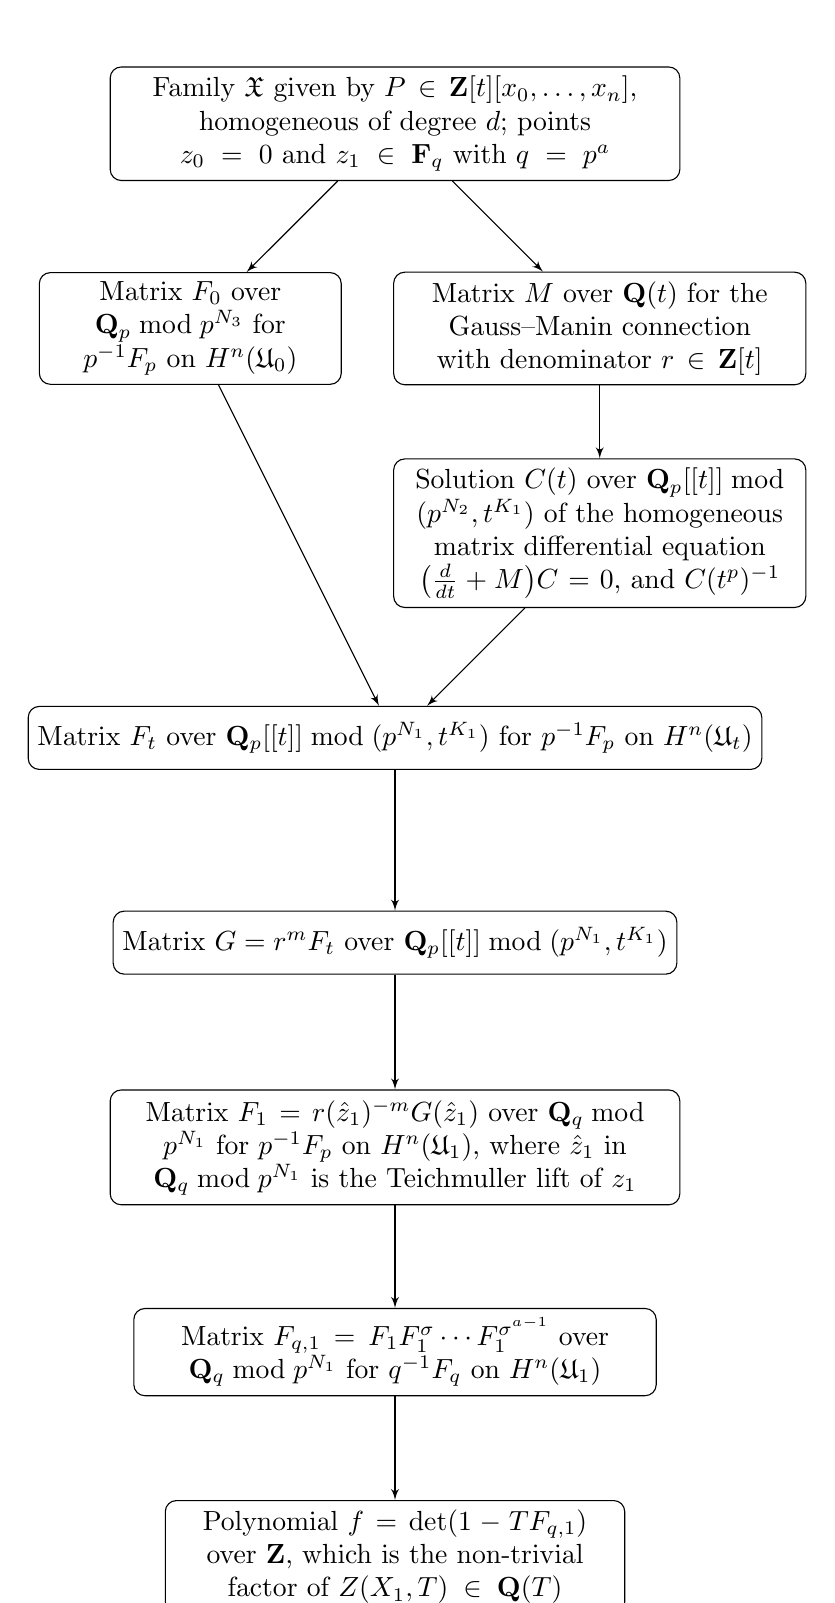
\begin{tikzpicture}[node distance = 2.6cm, auto]

    % Define block styles
    \tikzstyle{block} = [rectangle, draw, 
        text centered, rounded corners, minimum height = 8mm]
    \tikzstyle{empty} = [rectangle]
    \tikzstyle{line} = [draw, -latex']

    % Place nodes
    \node [block, text width = 70mm] (input) 
        {Family $\mathfrak{X}$ given by $P \in \mathbf{Z}[t][x_0, \dotsc, x_n]$, 
        homogeneous of degree $d$; 
        points $z_0 = 0$ and $z_1 \in \mathbf{F}_q$ with $q = p^a$};
    \node [empty, below of=input] (blah11) {};
    \node [block, left of=blah11, text width = 36mm] (diag) 
        {Matrix $F_0$ over $\mathbf{Q}_p \bmod p^{N_3}$ for $p^{-1} F_p$ 
        on $H^n(\mathfrak{U}_0)$};
    \node [block, right of=blah11, text width = 50mm] (gm) 
        {Matrix $M$ over $\mathbf{Q}(t)$ for the Gauss--Manin connection 
        with denominator $r \in \mathbf{Z}[t]$};
    \node [empty, below of=blah11] (blah21) {};
    \node [empty, left of=blah21] (blah20) {};
    \node [block, right of=blah21, text width = 50mm] (local) 
        {Solution $C(t)$ over $\mathbf{Q}_p[[t]] \bmod {(p^{N_2}, t^{K_1})}$ of the 
        homogeneous matrix differential equation $\bigl(\tfrac{d}{dt} + M\bigr) C = 0$, 
        and $C(t^p)^{-1}$};
    \node [block, below of=blah21] (series)
        {Matrix $F_t$ over $\mathbf{Q}_p[[t]] \bmod {(p^{N_1}, t^{K_1})}$ for $p^{-1} F_p$ 
        on $H^n(\mathfrak{U}_t)$};
    \node [block, below of=series] (poly) 
        {Matrix $G = r^m F_t$ over $\mathbf{Q}_p[[t]] \bmod {(p^{N_1}, t^{K_1})}$};
    \node [block, below of=poly, text width = 70mm] (eval) 
        {Matrix $F_1 = r(\hat{z}_1)^{-m} G(\hat{z}_1)$ over $\mathbf{Q}_q \bmod p^{N_1}$
        for $p^{-1} F_p$ on $H^n(\mathfrak{U}_1)$, 
        where $\hat{z}_1$ in $\mathbf{Q}_q \bmod p^{N_1}$ is the Teichmuller lift of $z_1$};
    \node [block, below of=eval, text width = 64mm] (qpower) 
        {Matrix $F_{q,1} = F_1 F_1^{\sigma} \dotsm F_1^{\sigma^{a-1}}$ 
        over $\mathbf{Q}_q \bmod {p^{N_1}}$ for $q^{-1} F_q$ on $H^n(\mathfrak{U}_1)$};
    \node [block, below of=qpower, text width = 56mm] (zeta) 
        {Polynomial $f = \det(1 - T F_{q,1})$ over $\mathbf{Z}$, 
        which is the non-trivial factor of $Z(X_1,T) \in \mathbf{Q}(T)$};

    % Draw edges
    \path [line] (input) -- (diag);
    \path [line] (input) -- (gm);
    \path [line] (gm) -- (local);
    \path [line] (diag) -- (series);
    \path [line] (local) -- (series);
    \path [line] (series) -- (poly);
    \path [line] (poly) -- (eval);
    \path [line] (eval) -- (qpower);
    \path [line] (qpower) -- (zeta);

\end{tikzpicture}
\caption{Flowchart describing the deformation algorithm}
\label{fig:deformation}
\end{figure}

\section{Precision estimates}

Most of the $p$-adic computations involved in the deformation 
method can only be carried out to finite precision, which means 
that we need to be able to effectively bound the $p$-adic 
precision lost during the various steps.  Determining the precison 
that we require for the final computation and working backwards 
through the algorithm, we find the precision required at 
each step.

\subsection{Computing Weil polynomials}

Recall that the zeta function of $X_1$ is of the form,
\begin{equation*}
Z(X_1,T) = \frac{p(T)^{(-1)^n}}{(1 - T) (1 - qT) \dotsm (1 - q^{n-1}T)}
\end{equation*}
where $p(T) = \det \bigl( 1 - T q^{-1} F_q | H^n(\mathfrak{U}_1) \bigr)$ 
is a polynomial defined over the integers.

In the final step of the deformation method, we compute the 
reverse characteristic polynomial $f(T)$ of the matrix $F_{q,1}$, 
which represents $q^{-1} F_q$ on $H^n(\mathfrak{U}_1)$ to some finite 
$p$-adic precision~$N_0$.  Which precision is necessary in order to 
correctly recover the Weil polynomial $p(T)$ over the integers?

We explicitly combine Theorem~{3.2} from Gerkmann~\citep{Gerkmann2007} 
with an improvement suggested by Kedlaya~\citep[Lemma~1.2.3]{Kedlaya2011}
to obtain the following precision bounds:

\begin{thm}
In order to recover $p(T)$ over $\mathbf{Z}$ it suffices to compute 
$f(T)$ modulo~$p^N$ where 
\begin{equation*}
N > \begin{cases}
    2 & (q,n,d) = (2,2,3) \\
    4 & (q,n,d) = (2,2,4) \\
    5 & (q,n,d) = (2,2,5) \\
    1 & (q,n,d) = (3,2,3) \\
    \log_p \bigl( 2 b \floorts{b/2}^{-1} q^{\floor{b/2} (n - 1) / 2} \bigr) & \text{otherwise}
    \end{cases}
\end{equation*}
provided that $\varepsilon = \sgn(\det(q^{-1} F_q))$ is known.
\end{thm}

\begin{proof}
Let us write the reverse characteristic polynomial of $q^{-1} F_q$ as 
\begin{equation*}
p(T) = \sum_{i=0}^{b} a_i T = \prod_{j=1}^{b} (1 - \alpha_j T).
\end{equation*}
We first recall three properties guaranteed by the Weil conjectures:
\begin{enumerate}
\item The map $\alpha \mapsto q^{n-1} \alpha^{-1}$ permutes the roots of $p(T)$.
\item The roots $\alpha_j$ have absolute value $\abs{\alpha_j} = q^{(n-1)/2}$.
\item The zeta function satisfies a function equation, which in terms of 
      the coefficients $a_0, \dotsb, a_b$ yields, for $0 \leq i \leq b$, 
      \begin{equation*}
      a_{b-i} = (-1)^b \varepsilon q^{(n-1) (b/2 - i)} a_i.
      \end{equation*}
\end{enumerate}

We now define the power sums $s_i$, for $i \geq 1$, 
\begin{equation*}
s_i = \alpha_{1}^i + \dotsb + \alpha_{b}^i
\end{equation*}
which satisfy the Newton identities 
\begin{equation*}
s_i + a_1 s_{i-1} + \dotsb a_{i-1} s_1 + i a_i = 0.
\end{equation*}
In particular, $s_i$ is an integer and 
$\abs{s_i} \leq b \max_j{\abs{\alpha_j}}^i = b q^{i(n-1)/2}$.
Assuming that we know $a_1, \dotsc, a_{i-1}$ and $s_1, \dotsc, s_{i-1}$ 
exactly, we can determine $s_i$ as an integer provided we know 
$i a_i$ modulo~$p^N$ with \mbox{$p^N > 2 b q^{i(n-1)/2}$}.

Using the functional equation to relate $a_{i}$ and $a_{b-i}$ 
and knowing the sign~$\varepsilon$, we can compute the top half 
of the coefficients once we have found $a_i$ for 
$0 \leq i \leq \floorts{b/2}$.

Thus, we can recover $p(T)$ as a polynomial over the integers 
from its residue modulo~$p^N$ where 
\begin{equation*}
p^N > \max \biggl\{ \frac{2b q^{k(n-1)/2}}{k} : 0 \leq k \leq \floorts{b/2} \biggr\}.
\end{equation*}

We observe that the sequence $\gamma_k = k^{-1} q^{k (n - 1) / 2}$ 
with $k \geq 1$ is increasing unless $(q,n)$ equals $(2,2)$ or $(3,2)$.  
In these remaining two cases, 
\begin{align*}
\gamma_3 & < \gamma_2 = \gamma_4 < \gamma_5 < \gamma_6 < \gamma_1 < \gamma_7 < \dotsc & (q,n) & = (2,2) \\
\gamma_2 & < \gamma_1 = \gamma_3 < \gamma_4 < \dotsc & (q,n) & = (3,2)
\end{align*}
Thus, we obtain the condition that 
\begin{equation*}
N > \begin{cases}
    2 & (q,n,d) = (2,2,3) \\
    4 & (q,n,d) = (2,2,4) \\
    5 & (q,n,d) = (2,2,5) \\
    1 & (q,n,d) = (3,2,3) \\
    \log_p \bigl( 2 b \floorts{b/2}^{-1} q^{\floor{b/2} (n - 1) / 2} \bigr) & \text{otherwise}
    \end{cases}
\end{equation*}
\end{proof}

\begin{rem}
We observe that $\varepsilon = \sgn(\det(q^{-1} F_q)) = 1$ whenever $b$ is even.

Indeed, from the Weil conjectures, we know that $\alpha \mapsto q^{n-1} \alpha^{-1}$ 
is a permutation of the roots.  Since it is a self-inverse, it partitions the 
set of roots into pairs and hence we can evaluate the product of the roots,
\begin{equation*}
a_b = \prod_{j=1}^{b} \alpha_j = q^{(n-1)b/2}.
\end{equation*}
Using the functional equation to relate $a_0 = 1$ and $a_b$, 
\begin{equation*}
a_{0} = (-1)^{b} \varepsilon q^{-(n-1) b / 2} a_{b}
\end{equation*}
it follows that $\varepsilon = (-1)^b$, which is equal to $1$ if $b$ is even.
\end{rem}

\begin{rem}
Moreover, $b$ is odd if and only if $n$ is odd and $d$ is even, which leaves 
one quarter of the cases to consider.  We suggest two possible ways in which 
one can arrive at a generic and provably correct implementation.

The first approach is to follow the above proof without making use of the 
functional equation, instead using the analogous precision estimate for the 
top coefficient~$a_b$.  This approach roughly doubles the number of $p$-adic 
digits that are required.  Specifically, the analogous result is to require 
\begin{equation*}
N > \begin{cases}
    2 & (q,n,d) = (2,2,3) \\
    5 & (q,n,d) = (2,2,4) \\
    1 & (q,n,d) = (3,2,3) \\
    \log_p \bigl( 2 q^{b (n-1) / 2} \bigr) & \text{otherwise}
    \end{cases}
\end{equation*}

An alternative approach is to first compute an $i' > \floorts{b/2}$ such 
that \mbox{$a_{i'} \neq 0$}.  This can be achieved, for example, by going 
through the entire deformation procedure to compute the reverse characteristic 
polynomial modulo~$p$ only.  In a second pass one then uses the analogous 
precision estimate obtained from the above proof for $a_{i'}$ in order to 
correctly determine the coefficients 
$a_0, \dotsc, a_{\floor{b/2}}, \dotsc, a_{i'}$.  Finally, the functional 
equation can be used to related $a_{b-i'}$ and $a_{i'}$ in order to determine 
$\varepsilon$.
\end{rem}

\subsection{Computing characteristic polynomials}

In this section we address the precision loss when computing the reverse 
characteristic polynomial $\det(1 - t A)$ of a $b \times b$ matrix $A$ 
given to finite precision over $\mathbf{Q}_p$.

From the definition of the determinant, 
\begin{align*}
\det(1 - t A) & = \sum_{\sigma \in S_b} \sgn(\sigma) 
                    \prod_{i=1}^{b} (1 - t A)_{i,\sigma(i)} \\
              & = \sum_{\sigma \in S_b} \sgn(\sigma) 
                    \prod_{i=1}^{b} \bigl( \delta_{i,\sigma(i)} - t A_{i,\sigma(i)} \bigr)
\end{align*}
where $S_b$ is the permutation group on $\{1,\dotsc,b\}$ and $\delta_{i,j}$ 
is equal to $1$ or $0$ as $i = j$ or $i \neq j$, respectively.

\begin{prop} \label{prop:productval}
Let $x_1, \dotsc, x_{\ell} \in \mathbf{Q}_p$, where $\ell \geq 2$, 
be given as $x_i = p^{v_i} u_i$ with $v_i = \ord_p(x_i) \in \mathbf{Z}$ 
and $u_i \in \mathbf{Z}_p^{\times}$ whenever $x_i \neq 0$ and 
$u_i = v_i = 0$ otherwise.  Suppose that $N \in \mathbf{Z}$ is given 
such that $N > \sum_{j=1}^{\ell} v_j$ and, for all $i$, $N > \sum_{j \neq i} v_j$.

Let $\tilde{x}_1, \dotsc, \tilde{x}_{\ell}$ be $p$-adic approximations 
satisfying $\ord_p(x_i - \tilde{x}_i) \geq N - \sum_{j \neq i} v_j$ 
for all $i$.  Then 
\begin{equation*}
\ord_p(x_1 \dotsm x_{\ell} - \tilde{x}_1 \dotsm \tilde{x}_{\ell}) \geq N.
\end{equation*}
\end{prop}

\begin{proof}
First, note that $x_i \neq 0$ implies that $\tilde{x}_i \neq 0$. 
Otherwise, if $\tilde{x}_i = 0$ then
\begin{equation*}
N - \sum_{j \neq i} v_j \leq \ord_p(x_i - \tilde{x}_i) = \ord_p(x_i) = v_i
\end{equation*}
which implies that $N \leq \sum v_j$, a contradiction.

Represent $\tilde{x}_i$ as $p^{\tilde{v}_i} \tilde{u}_i$ with the 
same convention that $\tilde{u}_i \in \mathbf{Z}_p^{\times}$ unless 
$\tilde{x}_i = 0$, in which case $\tilde{u}_i = \tilde{v}_i = 0$.  
We first show that $v_i = \tilde{v}_i$ whenever $x_i \neq 0$.  Indeed, 
if $v_i \neq \tilde{v}_i$ then 
\begin{equation*}
\ord_p(x_i - \tilde{x}_i) = \min\{\ord_p(x_i), \ord_p(\tilde{x}_i)\} \leq \ord_p(x_i) = v_i
\end{equation*}
whereas from the assumptions we derive 
\begin{equation*}
\ord_p(x_i - \tilde{x}_i) \geq N - \sum_{j \neq i} v_j > v_i,
\end{equation*}
a contradiction.

Note that, for all $i$ such that $x_i \neq 0$, the assumption 
$\ord_p(x_i - \tilde{x}_i) \geq N - \sum_{j \neq i} v_j$ implies that 
$\ord_p(u_i - \tilde{u}_i) \geq N - \sum_j v_j$.  Specifically, 
\begin{equation*}
\ord_p(u_i - \tilde{u}_i) = \ord_p(x_i - \tilde{x}_i) - v_i \geq N - \sum_{j=1}^{\ell} v_j.
\end{equation*}

Considering the product $x_1 \dotsm x_{\ell}$, we distinguish two 
cases.  First, assume that $x_i \neq 0$ for all $i$.  We find that 
\begin{equation*}
\ord_p(x_1 \dotsm x_{\ell} - \tilde{x}_1 \dotsm \tilde{x}_{\ell}) = 
    \sum_{j} v_j + \ord_p(u_1 \dotsm u_{\ell} - \tilde{u}_1 \dotsm \tilde{u}_{\ell}) \geq N.
\end{equation*}
In the other case, suppose that for some $k < \ell$, $x_1, \dotsc, x_k$ 
are non-zero and that $x_{k+1}, \dotsc, x_{\ell}$ are all zero.  In 
particular, $v_{k+1} = \dotsb = v_{\ell} = 0$.  Then 
\begin{equation*}
\begin{split}
\ord_p(x_1 \dotsm x_{\ell} - \tilde{x}_1 \dotsm \tilde{x}_{\ell}) 
  & = \ord_p(\tilde{x}_1 \dotsm \tilde{x}_{\ell}) \\
  & \geq v_1 + \dotsb + v_k + N - \sum_{j \neq k+1} v_j + \dotsb + N - \sum_{j \neq \ell} v_j \\
  & = (\ell - k) N - (\ell - k - 1) (v_1 + \dotsb + v_k) \\
  & > N. \qedhere
\end{split}
\end{equation*}
\end{proof}

\begin{cor}
Let $A$ be a $b \times b$ matrix over $\mathbf{Q}_p$ 
where $b \geq 2$.  With the same notation as in the 
previous Proposition, suppose that $N \in \mathbf{Z}$ 
satisfies, for all $\sigma \in S_b$ and $i$, 
\begin{equation*}
N > \sum_{j=1}^{b} v_{j,\sigma(j)}, \quad N > \sum_{j \neq i} v_{j,\sigma(j)}.
\end{equation*}
Assume that $\tilde{A}$ is an approximation to $A$
satisying, for all $\sigma \in S_b$ and $i$, 
\begin{equation*}
\ord_p \bigl(A_{i,\sigma(i)} - \tilde{A}_{i,\sigma(i)}\bigr) \geq N - \sum_{j \neq i} v_{j,\sigma(j)}.
\end{equation*}
Then 
\begin{equation*}
\ord_p\bigl( \det(1 - t A) - \det(1 - t \tilde{A}) \bigr) \geq N.
\end{equation*}
\end{cor}

\begin{rem}
In particular, if $\ord_p(A) = \ord_p(\tilde{A}) = -v < 0$ and 
$\ord_p(A - \tilde{A}) \geq N + (b - 1) v$ with $N$ satisfying 
the assumptions of the previous Corollary, then 
$\ord_p\bigl(\det(1 - t A) - \det(1 - t \tilde{A})\bigr) \geq N$.
\end{rem}

However, the matrices that we are interested in are far from generic 
as they represent the action of Frobenius and much better bounds are 
available.  The following result applies in the most general situation 
that we consider:

\begin{lem} \label{lem:charpoly}
Let $A$ denote the matrix representing the action of $q^{-1} F_q$ 
on $H^n(U)$ with respect to the monomial basis.  Define two 
integers $r$ and $s$ via \mbox{$r = \ord_p((n-1)!)$} and 
\mbox{$s = (n + 1) \floorts{\log_p (n-1)}$} and suppose that 
$A$ and $\tilde{A}$ are $p$-adically close, $\ord_p(A-B) \geq N + (r + s)$.  
Then 
\begin{equation*}
\ord_p \bigl( \det(1 - t A) - \det(1 - t \tilde{A}) \bigr) \geq N.
\end{equation*}
\end{lem}

\begin{proof} 
See Gerkmann~\citep[Lemma~3.3, Lemma~3.4]{Gerkmann2007}.
\end{proof}

\begin{rem}
As a consequence of Lemma~\ref{lem:charpoly}, we can take 
$N_1 = N_0 + r + s$ in our description of the deformation 
algorithm.

In particular, note that in the case that the prime~$p$ 
satisfies $p > n - 1$ we can choose $r = s = 0$ and there 
is no precision loss in this step of the computation.
\end{rem}

\subsection{Computing the action of $q^{-1} F_q$ on $H(\mathfrak{U}_1)$}

Let $F_1$ and $F_{q,1}$ denote the matrices representing the 
actions of $p^{-1} F_p$ and $q^{-1} F_q$ on $H(\mathfrak{U}_1)$, 
respectively.  By Gerkmann~\citep[Lemma~3.3]{Gerkmann2007}, 
the $p$-adic valuation of both matrices is bounded below by $-(r+s)$.  
We aim to compute $F_{q,1}$ via 
\begin{equation*}
F_{q,1} = F_1 F_1^{\sigma} \dotsm F_1^{\sigma^{a-1}}.
\end{equation*}

Since there is no precision loss involved in applying $\sigma$ [[TODO: Reference]], 
we can indeed compute $F_{q,1} \bmod p^{N_1}$ from $F_1 \bmod p^{N_1}$ 
by computing the product exactly over $\mathbf{Q}_p$ and only reducing 
modulo $p^{N_1}$ at the end.

\subsection{Analytic continuation and evaluation}

The matrix~$F_t$ is computed as matrix of power series in the first place 
by finding the local expansion of the solution to the differential equation 
around~$t = 0$.  Wishing to evaluate its entries at a point different 
from~$0$, we are prompted to compute its analytic continuation, that is to say, 
express the entries as rational functions instead of power series.

[[TODO:  Mention previously existing bounds by Gerkmann.]]

[[TODO:  Something about Jan and Kiran's paper, giving details about 
provable choices of $m$ and $K_1$.]]

\begin{rem}
Typically, the contribution of the terms 
$\max_i \lambda_i - p \min_i \lambda_i$ in Equation~[[TODO: Ref]] is small 
compared to $p g(N_1)$.  Therefore, in a simplified heuristic implementation, 
one can choose $m = 1.1 \times p N_1$ and $K_1 = (\deg(r) + 1) m$.
\end{rem}

The matrix $F_1$ is defined as the matrix of $p^{-1} F_p$ 
on $H(\mathfrak{U}_1)$ and it is computed as 
\begin{equation*}
F_1 = r(\hat{z}_1)^{-m} G(\hat{z}_1) \pmod{p^{N_1}}.
\end{equation*}
We claim that it suffices to compute 
$\hat{z}_1$ and $G$ to precision $p^{N_1}$.  Indeed, by 
assumption $r(z_1)$ is non-zero in $\mathbf{F}_p$ and so 
$r(\hat{z}_1)$ has valuation~$0$.  Therefore, $r(\hat{z}_1)^{-m}$ 
has valuation~$0$ and can be computed modulo $p^{N_1}$ 
without precision loss.

The matrix $G$ is computed as $G = r^m F_t$ over $\mathbf{Q}_p[[t]]$ 
modulo~$(p^{N_1}, t^{K_1})$.

\subsection{Local expansion}

From the previously computed pieces of data, that is, the 
matrix~$F_0$ representing $p^{-1} F_p$ on $H(\mathfrak{U}_0)$ 
and the matrix~$C(t)$ giving the solution to the homogeneous 
matrix differential equation, we can compute the matrix~$F(t)$ 
as 
\begin{equation} \label{eq:genfrob}
F(t) = C(t) F_0 C(t^p)^{-1}.
\end{equation}
Note that we wish to compute $F(t)$ modulo $(p^{N_1}, t^{K_1})$.

Regarding the $t$-adic precision, it is immediate that we 
need to compute $C(t)$ modulo $t^{K_1}$.  The third factor 
$C(t^p)^{-1}$ can be computed as $C(t)^{-1} \vert_{t=t^p}$, 
which requires us to compute $C(t)^{-1}$ modulo $t^{\ceil{K_1 / p}}$.

In order to establish bounds on the $p$-adic precision 
that require for the three factors, we need estimates of 
their $p$-adic denominators:

From~\citep[Lemma~3.3]{Gerkmann2007}, we know that the $p$-adic 
valuation of $F_0$ is bounded below by $-(r+s)$.

There are two bounds available in the literature that are 
relevant for the other two factors.  We begin by writing 
$C(t) = \sum_{i=0}^{\infty} C_i t^i$ with $C_i$ a matrix 
over $\mathbf{Q}_p$.  The first result we present can be 
found in the work of Lauder~[[TODO: Add Lauder Reference]] 
and Gerkmann~\citep[Theorem~5.1]{Gerkmann2007}.

\begin{thm}
The $p$-adic valuation of the $b \times b$ matrix $C_t$ is 
bounded from below by 
\begin{equation*}
\ord_p(C_i) \geq - \bigl( (b-1) + \ord_p((b-1)!) + 
    \min\{b-1,\ord_p \prod_j \binom{b}{j}\} \floor{\log_p(i)}.
\end{equation*}
\end{thm}

An improvement to this can be found in the work of 
Kedlaya~\citep[Theorem~18.3.3]{Kedlaya2010}.

[[TODO:  Develop a useful bound from Kedlaya's book.  Note that 
the factor $(1 - n)$ in the following result is likely to be 
wrong and will have to include something like $-(r + s)$.]]

\begin{thm}
\begin{equation*}
\ord_p(C_i) \geq (1 - n) \floor{\log_p{i}}.
\end{equation*}
\end{thm}

Consequently, we can bound the $p$-adic valuation of $C(t) \bmod t^{K_1}$ 
using the bound for $C_{K_1}$.  Similarly, by considering the differential 
equation 
\begin{equation*}
\bigl(d/dt - M^t\bigr) (C^{-1})^t = 0
\end{equation*}
we can bound the $p$-adic valuation of $C^{-1}(t^p)$.
\begin{cor}
The valuations of $C(t) \bmod{t^K}$ and $C^{-1}(t^p) \bmod{t^K}$ 
\end{cor}

With these bounds on the valuations for the three factors in 
Equation~\eqref{eq:genfrob} we aim to determine the values for 
$N_2$ and $N_3$ in the deformation method.

We have an analogous result to Proposition~\ref{prop:productval} 
for products of matrices:

\begin{prop} \label{prop:matrixproductval}
Let $A_1, \dotsc, A_{\ell}$ be $b \times b$ matrices over $\mathbf{Q}_p$, 
where $\ell \geq 2$, given as $A_i = p^{v_i} U_i$ with 
$v_i = \ord_p(A_i) \in \mathbf{Z}$ and at least one entry of $U_i$ a 
$p$-adic unit $A_i \neq 0$ and $v_i = 0$ and $U_i$ the zero matrix 
otherwise.  Suppose that $N \in \mathbf{Z}$ is given such that 
$N > \sum_{j=1}^{\ell} v_j$ and, for all $i$, $N > \sum_{j \neq i} v_j$.

Let $\tilde{A}_1, \dotsc, \tilde{A}_{\ell}$ be $p$-adic approximations 
satisfying $\ord_p(A_i - \tilde{A}_i) \geq N - \sum_{j \neq i} v_j$ 
for all $i$.  Then 
\begin{equation*}
\ord_p(A_1 \dotsm A_{\ell} - \tilde{A}_1 \dotsm \tilde{A}_{\ell}) \geq N.
\end{equation*}
\end{prop}

\begin{proof}
We can follow the proof of Proposition~\ref{prop:productval}, 
observing that, for matrices $A$, $B$ over $\mathbf{Q}_p$, 
we have $\ord_p(A + B) \geq \min \{\ord_p(A), \ord_p(B)\}$.
\end{proof}

[[TODO:  Determine actual values for $N_2$ and $N_3$, once we have 
corrected the bounds for $\ord_p(C_i)$.  Suppose that 
$\ord_p(C) \geq x$, $\ord_p(F_0) \geq y$, and $\ord_p(C^{-1}) \geq z$.]]

\begin{cor}
In order to compute the product $F(t) = C(t) F(0) C^{-1}(t^p)$ to 
precision $N_1$, we need to have $C(t)$, $F(0)$, and $C^{-1}(t^p)$ 
to precisions 
\begin{align*}
N_2  & \geq N_1 - y - z, \\
N_3  & \geq N_1 - x - z, \\
N_2' & \geq N_1 - x - y,
\end{align*}
respectively.
\end{cor}

\begin{proof}
This follows from Proposition~\ref{prop:matrixproductval}, observing 
that the bounds on the valuations of $C(t)$, $F(0)$, and $C^{-1}(t^p)$ 
are non-positive.
\end{proof}

[[TODO:  Working precisions for the local solution to the differential equation.]]

%%%%%%%%%%%%%%%%%%%%%%%%%%%%%%%%%%%%%%%%%%%%%%%%%%%%%%%%%%%%%%%%%%%%%%%%%%%%%%%
% Examples                                                                    %
%%%%%%%%%%%%%%%%%%%%%%%%%%%%%%%%%%%%%%%%%%%%%%%%%%%%%%%%%%%%%%%%%%%%%%%%%%%%%%%

\chapter{Examples}


}

{%
\part{The fibration method and fast radix conversion for polynomials}
\setlength{\baselineskip}{1.5\baselineskip}
%\include{fibration}
}

{%
\part{Implementation details}
\setlength{\baselineskip}{1.5\baselineskip}
%\include{arithmetic}
}

\backmatter

\phantomsection
\addcontentsline{toc}{chapter}{References}

\bibliographystyle{amsplain}
\bibliography{../SPancratz}

\end{document}

